\chapter{Оценка параметров ШАЛ}

В предыдущей главе описан метод байесовской деконволюции и его применение к данным эксперимента СФЕРА-2. В результате получена безмодельная оценка потоков фотонов на мозаике ФЭУ в том смысле, что она не зависит от детальных предположений о свойствах и источниках света, падающего на мозаику, кроме самых общих представлений. В этой главе на основе полученного результата, а также качественного представления о пространственно-временной структуре сигнала ШАЛ реконструируется функция пространственного распределения (ФПР) черенковского света. Наконец, на основе полученной ФПР делаются оценки параметров ШАЛ.

Стоит отметить, что методы, изложенные в этой главе, не являются инновационными сами по себе, напротив, использованы уже хорошо изученные подходы. Основной целью является демонстрация того, как эти методы работают в контексте эксперимента СФЕРА-2 с учётом описанной процедуры деконволюции и неопределённостей, которые она порождает.

\section{Выделение сигнала ШАЛ и оценка значимости}

В процессе деконволюции не делается предположений о наличии или отсутствии сигнала ШАЛ в исследуемой области экспериментального кадра. Из моделирования ливня и оптической системы эксперимента известен общий вывод -- фотоны ШАЛ достигают мозаики в виде \textit{пакетов} -- групп фотонов с приближённо нормальным распределением времён прихода. Каждый пакет можно описать тремя параметрами: $n_{EAS}$ -- суммарное число фотонов в пакете, $\mu_t$ -- среднее время прихода фотонов, $\sigma_t$ -- стандартное отклонение времён прихода. Ещё одним параметром является среднее число фоновых фотонов $\lambda_{n}$, однако, как показано в разделе \ref{sec:expdata-preparation-for-deconvolution}, оно известно из абсолютной калибровки сигнала.

\subsection{Выделение пакета фотонов ШАЛ}

\label{sec:signal-reconstruction}

Как и задача деконволюции (\ref{sec:bayesian-deconvolution-solution}), задача выделения сигнала ШАЛ может быть решена с помощью байесовского вывода. В качестве параметров модели используем $\Theta \equiv (n_{EAS}, \mu_t, \sigma_t)$, в качестве наблюдаемых данных -- полученную в результате деконволюции выборку значений $\vec{n}$.

Определим функцию правдоподобия для этой задачи: она должна давать вероятность того, что при фиксированном значении $\Theta$ будет получены наблюдаемое $\vec{n}$. То обстоятельство, что $\vec{n}$ измерен не прямо, а задан апостериорным распределением, легко учесть, просто усреднив значения функции правдоподобия по всем элементам этой выборки.

Представим $\vec{n}$ в виде суммы $\vec{n}_{EAS} + \vec{n}_{noise}$. Распределение случайного вектора $\vec{n}_{EAS}$ проще всего разыграть численно, генерируя выборки времён прихода фотонов объёмом $n_{EAS}$ из распределения $N(\mu_t, \sigma_t)$, и рассчитывая из них гистограмму в границах экспериментальных бинов. Для нахождения искомой функции правдоподобия остаётся вычислить вероятность того, что <<остаток>> $\vec{n}_{noise}$ имеет пуассоновское распределение с $\lambda_{n}$ в каждом бине:

\begin{equation}
	\mathcal{L}(\Theta) \equiv P(\vec{n} | n_{EAS}, \mu_t, \sigma_t) = \prod_{i} \frac{e^{-\lambda_n} \lambda_n^{n_{noise}^{(i)}}}{(n_{noise}^{(i)})!}
\end{equation}

Формула выше описывает значения правдоподобия при фиксированных $\vec{n}_{EAS}$ и  $\vec{n}$, поэтому для получения окончательного результата требуется усреднить значение $\mathcal{L}$ по соответствующим распределениям (флуктуациям гистограммы $\vec{n}_{EAS}$ и апостериорному распределению деконволюции).

В отличие от неинформативного априорного распределения, описанного для деконволюции в разделе \ref{sec:deconv-prior}, для $\Theta$ можно выбрать априорные распределения из данных моделирования. Известно, что $n_{EAS}$ для интересующего нас диапазона энергий в $1$ - $100$ ПэВ имеет априорное распределение, экспоненциально спадающее от нуля с показателем $\sim 40$, а $\sigma_t$ -- $N(2.4, 2)$ (в бинах). Для $\mu_t$ было выбрано априорное распределение, равномерное на ширине окна деконволюции \footnote{В будущем при развитии методики можно уже на этапе поиска пакета <<угадывать>> его предполагаемое положение из приближённой оценки ориентации плоскости ливня по нескольким самым ярким каналам, и вносить эту информацию в априорное распределение $\mu_t$.}. Использование информативных априорных распределений помогает в процессе сэмплирования быстрее <<навестись>> на нужные области, например, сразу отбросить слишком широкие или многочисленные пакеты как маловероятные.

Техническая реализация MCMC-сэмплирования полностью аналогична описанной в разделе \ref{sec:mcmc-sampling}.

\begin{figure}
	\centering
	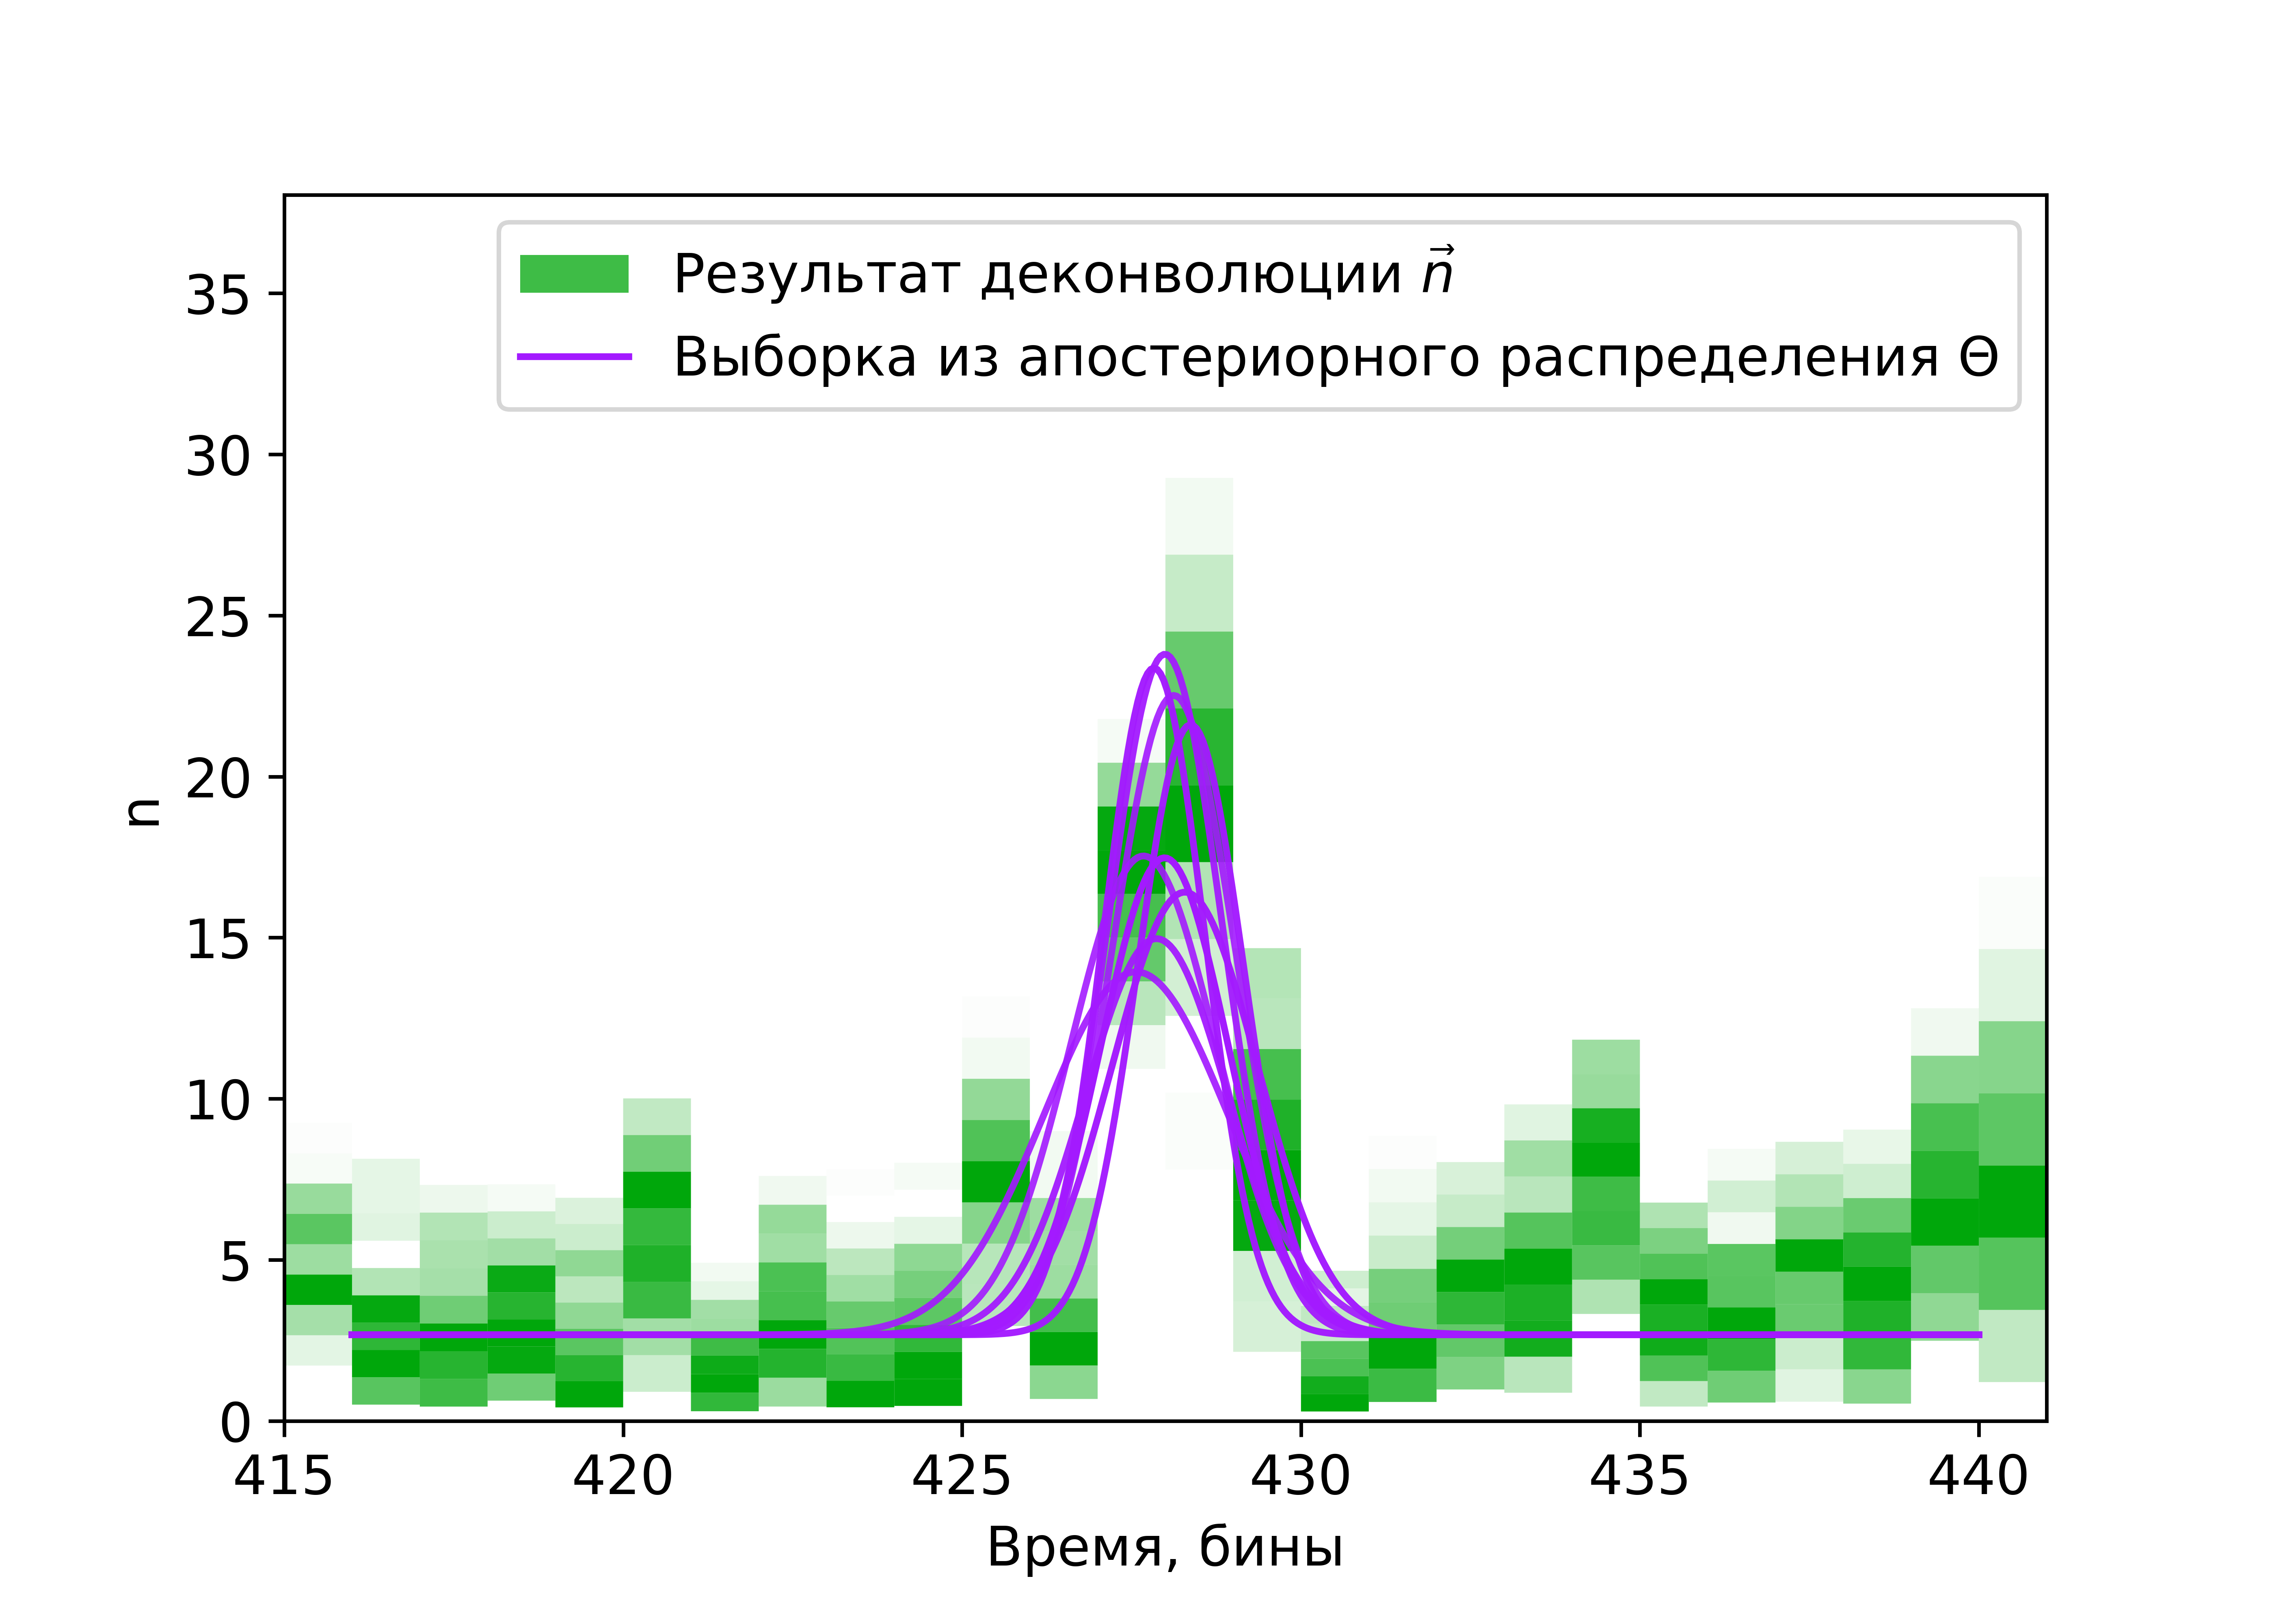
\includegraphics[width=\columnwidth]{signal-reconstruction-example}
	\caption{Выделение пакета фотонов ШАЛ из результатов байесовской деконволюции. Фиолетовыми кривыми представлены $10$ пакетов фотонов, соответствующих случайным элементам из апостериорной выборки $\Theta$ (см. текст). Видно, что пакеты группируются вблизи ожидаемого пика, но их параметры варьируются, учитывая неопределённость данных деконволюции.}
	\label{pic:signal-reconstruction-example}
\end{figure}


\subsection{Оценка значимости выделенного сигнала}

Одно из преимуществ полностью статистического подхода -- возможность использовать понятие значимости в процессе разделения сигнала ШАЛ и сигнала от фоновых фотонов. Широко принятый в байесовской статистике инструмент для этого -- байесовский информационный критерий (Bayesian information criterion, BIC), введённый Шварцем \cite{Schwarz1978} и в некотором смысле адаптирующий для байесовского анализа информационный критерий Акаике \cite{Akaike1974}. Суть его состоит в следующем: при наличии нескольких моделей, описывающих данные, их можно сравнить по количеству информации, которое теряется при замене данные на модель. Чем меньше значение критерия, тем лучше модель. Вычисление проводится по формуле

\begin{equation}
	\mathrm{BIC} = k \ln n - 2 \ln \mathcal{L}_{max}
\end{equation}

Здесь $k$ -- число параметров модели, $n$ -- число элементов выборки данных, $\mathcal{L}_{max}$ -- максимальное значение функции правдоподобия для данной модели. Структура выражения указывает на интуитивное качество критерия: чем больше число параметров модели $k$, тем больше требуемый прирост $\mathcal{L}_{max}$, это позволяет предотвратить переобучение модели с большим числом параметров.

Для определения значимости найденного сигнала ШАЛ нам нужно сравнить две модели: модель <<только шума>> ($n_{EAS} = 0$) вовсе без параметров ($k=0$), и модель <<шум + сигнал>>, описанную в предыдущем разделе, которая имеет $k=3$ параметра. По разнице $ \Delta \mathrm{BIC} = \mathrm{BIC}_{noise} - \mathrm{BIC}_{noise + EAS}$ можно судить о значимости восстановленного сигнала.

Если $\Delta \mathrm{BIC} \leq 0$, то модель только шума оказывается более состоятельной, и такой канал можно удалить из анализа. Если $0 < \Delta \mathrm{BIC} < 4$, то сигнал можно считать слабым, на практике оказывается, что в эту область чаще всего попадают артефакты деконволюции или флуктуации фона. Каналы, в которых $\Delta \mathrm{BIC} > 4$, принимались как достоверные (хотя и в этом случае иногда находятся артефакты, которые позже отсеиваются на этапе восстановления геометрии ливня).

На рис. \ref{pic:deconvolution-and-reconstruction} представлен пример сначала деконволюции, а затем восстановления параметров пакетов фотонов для экспериментального события. Оценка значимости сигналов использована, чтобы часть точек отсеить совсем, а часть пометить как <<сомнительные>>, однако видно, что в последних каналах присутствуют, по-видимому, артефакты деконволюции, которые дают ложные сигналы, но которые, впрочем, легко отделить по времени прихода. Тем не менее, наличие подобных ложных срабатываний затрудняет поиск истинных слабых сигналов ШАЛ, и способы борьбы с ними разрабатываются и будут применены в будущем.

\begin{figure}
	\centering
	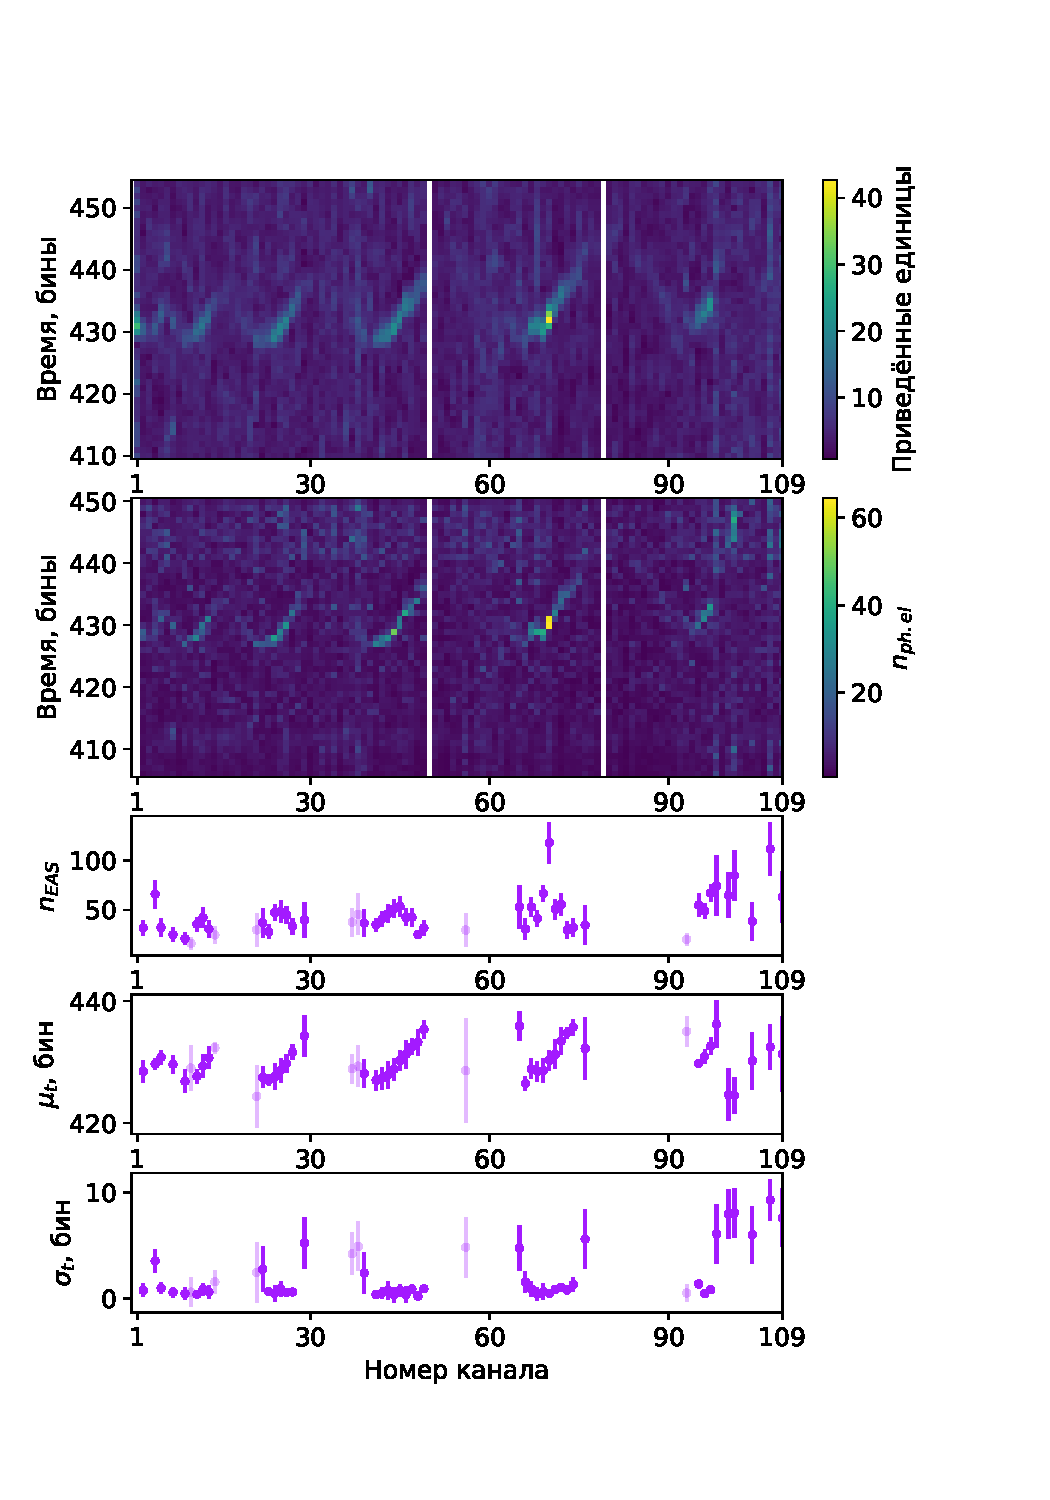
\includegraphics[width=0.86\columnwidth]{deconvolution-and-reconstruction}
	\caption{Деконволюция и восстановление параметров пакетов для экспериментального события \#10675. Для параметров $n_{EAS}, \mu_t, \sigma_t$ ярким цветом показаны точки со значениями $\Delta \mathrm{BIC} > 4$, тусклым -- $\Delta \mathrm{BIC} \in (0, 4]$, значения с отрицательным $\Delta \mathrm{BIC}$ исключены -- видно, что они соответствуют <<пустым>> областям кадра.}
	\label{pic:deconvolution-and-reconstruction}
\end{figure}


\section{Направление прихода ливня}

Стандартный метод оценки направления прихода (или, иначе, ориентации оси) ливня основан на представлении о том, что фронт черенковского света (а в случае с другими установками -- и заряженных частиц) с хорошей точностью является плоским. Поэтому, аппроксимируя экспериментально измеренную зависимость времени прихода фронта $\bar{t}_{gnd}(x, y)$, мы сразу получаем оценку углов ориентации вектора нормали.

Для обработки данных эксперимента СФЕРА-2 требуется сделать дополнительный шаг: учесть время распространения света от снега до детектора. Это легко сделать, учитывая, что для каждого ФЭУ известен центр его поля зрения на поверхности $(x_i, y_i)$ (см. раздел \ref{sec:light-collection-from-surface} и в частности рис. \ref{pic:experimental-pmt-fov-example}), и отсюда, зная высоту подъёма установки $H$, получаем $\bar{t}_{i} = \mu_t^{(i)} - \frac{\sqrt{H^2 + x_i^2 + y_i^2}}{c}$.

Задача аппроксимации трёхмерных точек плоскостью решается линейным методом наименьших квадратов, однако сам по себе этот метод неустойчив к выбросам, а, как видно на рис. \ref{pic:deconvolution-and-reconstruction}, выбросы в данных $\mu_t$ присутствуют. Для решения этой проблемы была разработана методика простого итеративного фитирования: аппроксимируется набор точек, находится самая удалённая от плоскости точка, выбрасывается, новый набор аппроксимируется заново, и так далее. Процедура повторяется до тех пор, пока угол между векторами нормали в двух последовательных аппроксимациях не станет меньше заданного наперёд значения. В настоящей работе это значение допустимого <<дрожания>> было положено равным $0.1$ градус. Следует заметить, что это не ограничение на погрешность определения ориентации оси, но только на устойчивость оптимального значения этой ориентации относительно удаления <<наихудшей>> точки. Погрешность определения углов $\theta$ и $\phi$ получалается естественным образом в процессе фитирования, зависит от числа точек и составляет в общем случае порядка нескольких градусов. На рис. \ref{pic:plane-reconstruction} показаны два примера этой процедуры для разных событий.


\begin{figure}
	\centering
	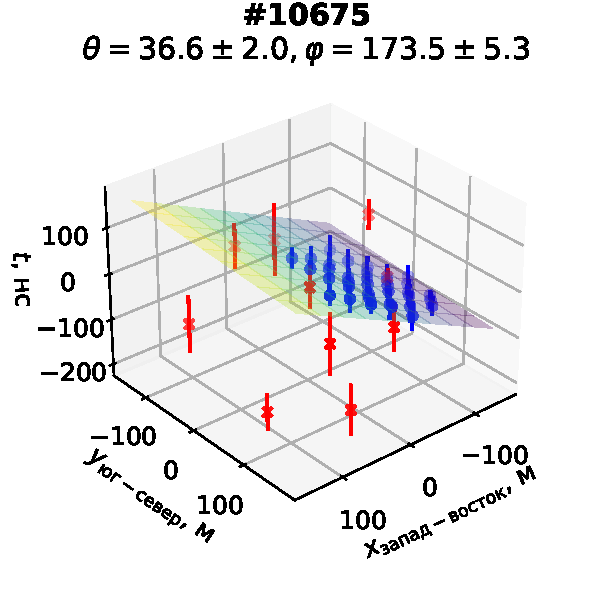
\includegraphics[width=0.45\columnwidth]{showe-plane-approximation-10675}
	\hfill
	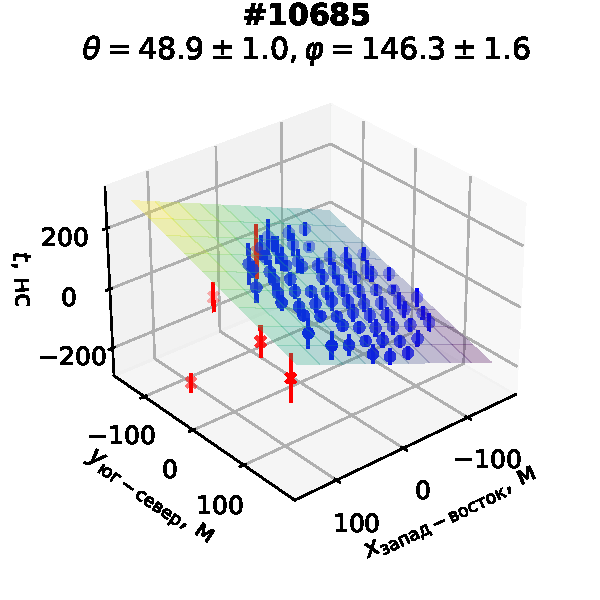
\includegraphics[width=0.45\columnwidth]{showe-plane-approximation-10685}
	\caption{Восстановление ориентации ШАЛ для двух экспериментальных событий. Красными показаны точки, автоматически исключённые в процессе итеративного фитирования (см. текст).}
	\label{pic:plane-reconstruction}
\end{figure}

\subsection{Перспективы уточнения оценки}

Описанный метод является стандартным и устоявшимся, однако может быть уточнён с учётом индивидуальных особенностей эксперимента СФЕРА-2. В бакалаврской дипломной работе (как сослаться на свою же?) был разработан метод уточнения оценки ориентации оси, рассматривающий ширину пакета фотонов как вторичный показатель. Идея метода основана на том, что для протяжённых полей зрения ФЭУ ожидается наличие зависимости $\sigma_t(x, y)$ -- для ФЭУ, через которые фронт ливня проходит первым, пакет фотонов будет \'{у}же, чем для расположенных на противоположной стороне мозаики. Этот <<геометрический эффект>> является следствием взаимной угла между падающим и рассеянным черенковским светом, и соответствующим сжатием или растяжением пакета во времени.

В настоящей работе такой анализ проведён не был.

\section{Положение оси ливня}

Для оценки положения оси ливня -- то есть координат её пересечения с поверхностью наблюдения можно использовать ряд методов; в этом разделе описан один из самый простых, основанный только на предположении о том, что функция пространственного распределения фотонов монотонно убывает с расстоянием от оси ливня.

Из восстановленных параметров пакетов фотонов в каждом канале мы имеем зависимость оценки $n_{EAS}$, найденной для каждого канала в разделе \ref{sec:signal-reconstruction}, от координат на поверхности наблюдения. К этому моменту мы исключили из рассмотрения каналы с низкой значимостью найденного сигнала, а также каналы, исключённые в процессе восстановления плоскости ливня (см. предыдущий раздел).

Сформулируем функцию правдоподобия, задающую вероятность того, что ось пересекает поверхность наблюдения в точке $(x_{ax}, y_{ax})$. Зная эти координаты, перенумеруем каналы по возрастанию расстояния от предполагаемого положения оси -- тогда функция правдоподобия будет равна вероятности того, что $\forall i, j: i < j$ будет выполняться $n_{EAS}^{(i)} > n_{EAS}^{(j)}$. Для простоты положим здесь и далее, что апостериорное распределение $n_{EAS}^{(i)}$ в $i$-том бине приближённо нормально и описывается только средним $\mu_i$ и стандартным отклонением $\sigma_i$.

\begin{equation}
	\mathcal{L}(x_{ax}, y_{ax}) = \prod_i \prod_{j > i} \left( 1 - F_{N}(0, \mu_i - \mu_j, \, \sqrt{\sigma_i + \sigma_j}) \right)
\end{equation}

Здесь $F_{N}(x, \mu, \sigma) = \frac{1}{2} \left[ 1 + \mathrm{erf} \left( \frac{x - \mu}{\sqrt{2 \sigma^2}} \right) \right]$ -- функция распределения гауссовой случайной величины, её параметры $\mu_i - \mu_j$ и $\sqrt{\sigma_i + \sigma_j}$ соответствуют распределению разности двух нормалных случайных величин, $1 - F_N(0)$ даёт вероятность того, что разность случайных величин больше нуля.

Эту функцию правдоподобия можно максимизировать для поиска наиболее вероятного положения оси. Следует заметить, что, так как в основе $\mathcal{L}$ лежит только представление о монотонности ФПР, но не о характере её зависимости от радиуса, область максимального правдоподобия будет иметь конечные размеры, в её пределах упорядочивание каналов по возрастанию расстояния от оси не будет изменяться, и функция правдоподобия будет иметь строго одинаковые значения. На практике оказалось, что область такого <<вырождения>> весьма мала, и метод пригоден по крайней мере для начальной оценки.

Более сложные методы могут восстанавливать положение оси не отдельным параметром, а вместе с формой ФПР, проводя общий трёхмерный фит. Для упрощения такие методы не были рассмотрены, но переход к ним не представляет концептуальной сложности.

\section{Восстановление функции пространственного распределения черенковского света}

После определения ориентации и положения оси ливня в пространстве можно приступить к оценке пространственного распределения черенковского света ШАЛ. Форма ФПР черенковского света представляет существенный интерес, так как даёт способ оценки параметров ливня, слабо зависящий от модели ядерного взаимодействия. В частности, нормировка ФПР даёт информацию об энергии ливня, а форма (часто измеряемая показателем наклона, определяемого как отношение потоков на двух радиусах), предоставляет некоторые возможности для определения массы первичной частицы ШАЛ \cite{Patterson1983, Dawson1989, TOKUNO2008}.

Полный обзор и сравнение разных аппроксимаций черенковской ФПР остаётся за рамками настоящей работы, в качестве показательного метода будем использовать двухпараметрическую функцию, разработанную для аппроксимации данных детекторов черенковского света в эксперименте Тунка-25 \cite{Budnev2005}:

\begin{equation}
	\label{eq:tunka-25-ldf}
	\begin{gathered}
	Q(R) = Q_{kn} \cdot \begin{cases}
		\exp \left( \frac{(R_{kn} - R) \cdot (1 + 3/(R+3))}{R_0} \right) \text{ при } R < R_{kn} \\
		\left(\frac{R_{kn}}{R}\right)^b \text{ при } R \geq R_{kn} 
	\end{cases} \\
	R_0 = 10^{2.95 - 0.245 P}, \text{м}  \\
	R_{kn} = 155 - 13P, \text{м} \\
	b = 1.19 + 0/23 P
	\end{gathered}
\end{equation}

Параметр $Q_{kn}$ задаёт нормировку ФПР, а $P$ -- параметр наклона, равный отношению $Q(100)/Q(200)$ -- определяет её форму.

Также стоит отметить, что возможен другой подход, основанный не на аналитической аппроксимации ФПР, а на прямом сравнении экспериментальных данных с ФПР, полученной из Монте-Карло симуляции ливня. Предполагается, что такой метод должен давать наибольшую точность, хотя и требовать больше вычислительных ресурсов. Вне зависимости от способа получения зависимости $Q(x, y)$ и количества её варьируемых параметров, способ сравнения с экспериментальными данными остаётся тем же.

\subsection{Проекция полей зрения ФЭУ на плоскость ливня}

В разделе \ref{sec:light-collection-from-surface} описан процесс получения <<полей зрения>> ФЭУ -- распределений коэффициентов сбора $f^{(i)}(x_{gnd}, y_{gnd})$ по отражающей поверхности под установкой. Однако функция $Q(x_{shw}, y_{shw})$ задаётся в плоскости ливня, поэтому требуется спроецировать $f^{(i)}$ на неё же.

Для этого учтём, что плоскость ливня задаётся нормалью $(\theta_{shw}, \varphi_{shw})$ в системе земли и для определённости пересекает поверхность земли в начале координат. На плоскости ливня можно ввести систему координат с горизонтальной осью $x_{shw}$, направленной <<слева-направо>> с точки зрения движущегося ливня, и осью $y_{shw}$, лежащей в одной плоскости с вертикалью (<<снизу-вверх>> с точки зрения ливня). Тогда для произвольной точки на поверхности земли, выраженной полярными координатами $(r_{gnd}, \varphi_{gnd})$ из простых геометрических соображений найдём $x_{shw} = - r_{gnd} \, \sin (\varphi_{shw} - \varphi_{gnd})$, $y_{shw} = - r_{gnd} \, \cos (\varphi_{shw} - \varphi_{gnd}) \, \cos \theta_{shw}$.

Таким образом спроецированные поля зрения дают суммарное распределение чувствительности установки $f(x_{shw}, y_{shw})$ в плоскости ливня. Пример такой проекции на ливень с зенитным углом падения $\approx 30^{\circ}$ приведён на рис. \ref{pic:projected-pmt-fov}. Заметим, что, так как функция $f$ является безразмерным коэффициентом сбора, нет необходимости учитывать преобразование элемента площади при проекции.

\begin{figure}
	\centering
	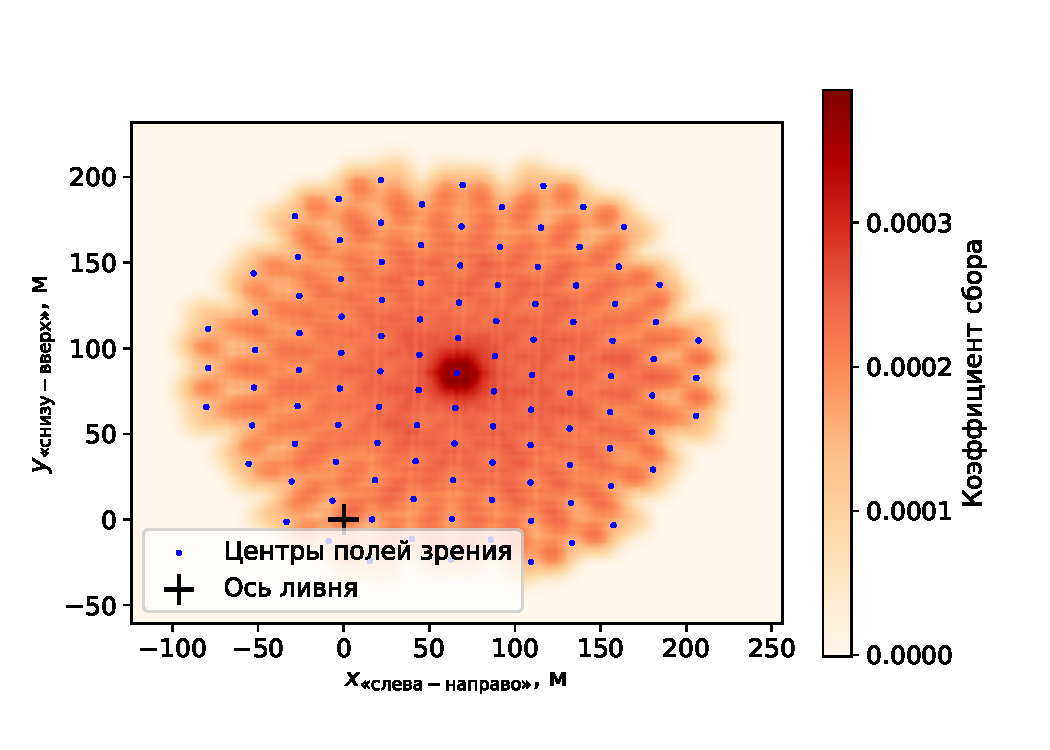
\includegraphics[width=\columnwidth]{projected-pmt-fov}
	\caption{Распределение чувствительности установки в плоскости фронта ливня.}
	\label{pic:projected-pmt-fov}
\end{figure}

\subsection{Преобразование фотонов черенковского света ШАЛ в эквивалентные фотоэлектроны}

До сих пор мы, как указано в разделе \ref{sec:photon-to-phels-conversion}, работали с количеством эквивалентных фотоэлектронов, рождённых сигналом ШАЛ на фотокатоде ФЭУ. Для построения ФПР черенковского излучения требуется описать, как происходит пересчёт одной величины в другую.

Заметим, что искомая величина плотности черенковского света измеряется \textit{на единицу энергии}: $Q(x, y)$ [$\text{фотоны} \cdot \text{м}^{-2} \cdot \text{эВ}^{-1}$] \cite{Budnev2005}, так как в соответствии с формулой Франка-Тамма \cite{Tamm1939} $dN _{\gamma}/dE \approx Const$ в видимой части спектра. Тогда зная квантовую эффективность ФЭУ $\kappa(E)$, а точнее её среднее значение $\bar{\kappa}$ в диапазоне энергий $[E_{min}, E_{min} + \Delta E]$, можно перейти от $Q$ к флюенсу эквивалентных фотоэлектронов $n_{ph. el.} (x, y)$ [$\text{фотоэлектроны} \cdot \text{м}^{-2}$]:

\begin{equation}
	\Delta E \; \bar{\kappa} Q(x, y) = n_{ph. el.}
\end{equation}

Кривые квантовой эффективности для двух видов ФЭУ приведены на рис. \ref{pic:pmt-quanteffs}. Коэффициент $\Delta E \; \bar{\kappa}$ составляет $0.34~\text{эВ}$ для Hamamatsu R3886 и $0.39~\text{эВ}$ для ФЭУ84-3.

\begin{figure}[H]
	\centering
	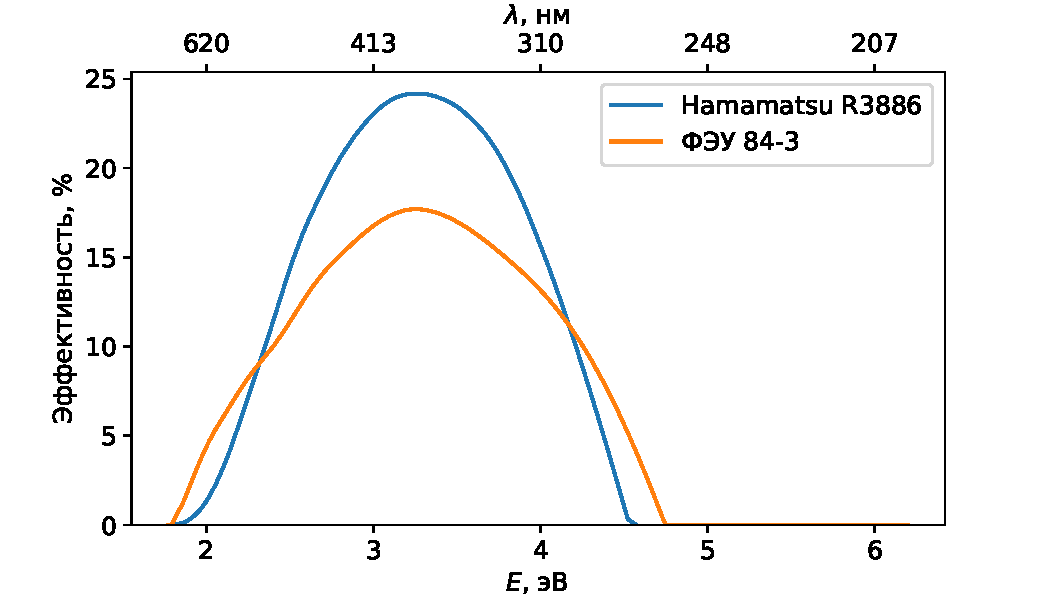
\includegraphics[width=\columnwidth]{pmt-quantum-efficiences}
	\caption{Кривые квантовой эффективности для двух видов ФЭУ, использованных в эксперименте СФЕРА-2}
	\label{pic:pmt-quanteffs}
\end{figure}


\subsection{Неопределённость сбора света со снега}

Учтём, что до сих пор мы получали апостериорную оценку на число фотоэлектронов, выбитых с фотокатода ФЭУ под действием фотонов ШАЛ. В то же время из модели мы можем получить только математической ожидание этой величины, но не её точное значение -- процесс сбора света сам является стохастическим. Хорошим приближением для него является пуассоновское распределение. Иначе говоря, если среднее число фотонов, ожидаемое к $i$-том канале, равно $\lambda^{(i)}$, то реально зарегистрировано будет $n^{(i)} \sim \mathrm{Poisson}(\lambda^{(i)})$. Таким образом нам необходимо, зная апостериорное (относительно процесса деконволюции, выделения пакета фотонов и т.д.) распределение $n$, нужно получить оценку $\lambda$ (индекс канала $i$ опущен).

Для этого рассмотрим случай, когда $n$ известно точно. Тогда теорема Байеса в <<вырожденном>> виде сразу даёт апостериорное распределение $\lambda$:

\begin{equation}
	P(\lambda | n) = P(n | \lambda) = \frac{e^{-\lambda} \lambda^n}{n!}
	\label{eq:lmbda-posterior-precise}
\end{equation}

Иначе говоря, плотность апостериорного распределения непрерывной величины $\lambda$ задаётся той же формулой, что и само распределение пуассона, но где $\lambda$ является аргументом, а $n$ -- параметром.

Теперь перейдём к случаю, где $n$ не известно точно, но имеет некоторое распределение. Учитывая, что $n$ может принимать только целые значения, представим выборку из апостериорного распределения в виде таблицы частотности: $\lbrace n_i, p_i \rbrace, i = 1, ..., k$, где $p_i$ -- вероятность, что $n$ имеет значение $n_i$. Тогда ясно, что апостериорное распределение $\lambda$ будет равно дискретной <<свёртке>> выражения (\ref{eq:lmbda-posterior-precise}) с распределением $n$:

\begin{equation}
P(\lambda) = \sum_{i=1}^{k} p_i \frac{e^{-\lambda} \lambda^{n_i}}{n_i !}
\end{equation}

На практике оказывается, что такая свёртка уширяет и так достаточно широкое апостериорное распределение $n$ сравнительно не сильно -- до $10$ -- $20 \%$.


\subsection{Аппроксимация ФПР}

Пользуясь результатами педыдущих двух разделов, запишем окончательное выражение для ожидаемого среднего числа фотоэлектронов от света ШАЛ, зарегистрированных в $i$-том ФЭУ.

\begin{equation}
	\int_{\infty} f^{(i)}(x, y)
	; \Delta E \; \bar{\kappa} \; Q(x, y) \; dx dy = \lambda_n^{(i)}
\end{equation}

Интегрирование можно провести численно по известным точкам распределения $f^{(i)}(x, y)$ в плоскости ливня. Используя данные апостериорного распределения $\lambda_n^{(i)}$, можно найти среднее значение и стандартное отклонение этой величины для использования в аппроксимации.

Визуализировать такое фитирование в традиционных координатах $R, Q(R)$ непросто, так как величина $Q(R)$ сворачивается с двумерной функцией распределения чувствительности для каждого ФЭУ. Приближённую качественную картину можно получить, если пренебречь протяжённостью полей зрения и считать, что они достаточно малы, чтобы можно было положить $Q(x, y) = Const = Q(x_c, y_c)$: $\Delta E \; \bar{\kappa} \; Q(x_c, y_c) \int_{\infty} f^{(i)}(x, y) \; dx dy = \lambda_n^{(i)}$. Такая визуализация приведена на рис. \ref{pic:ldf-fit-example-1} и \ref{pic:ldf-fit-example-2}, однако следует подчеркнуть её неточность. В частности за счёт протяжённых полей зрения, эксперимент СФЕРА-2 чувствителен к черенковскому свету в приосевой области, поэтому точность и устойчивость фита заметно выше, чем может показаться по этим упрощённым графикам. Также точность повышается за счёт наложения полей зрения ФЭУ -- в некоторых областях поверхности свет регистрируется сразу двумя или даже тремя ФЭУ, что эффективно уменьшает погрешности определения $\lambda_n$ в них.


\begin{figure}
	\centering
	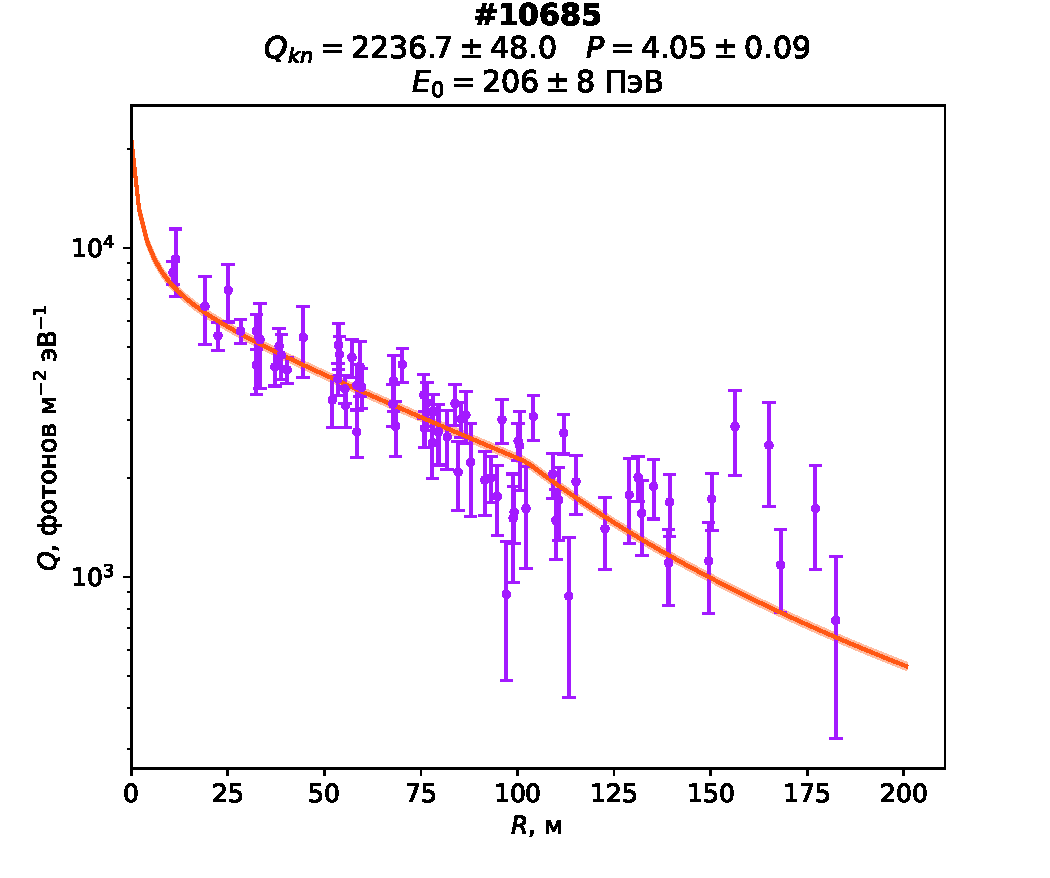
\includegraphics[width=0.9\columnwidth]{ldf-fit-10685}
	\caption{Упрощённая визуализация фитирования ФПР по данным эксперимента СФЕРА-2 (см. текст). Погрешность определения нормировки $Q_{kn}$ показана на графике коридором вокруг наиболее вероятной теоретической ФПР. Инструментальная погрешность определения энергии вычислена по формуле (\ref{eq:E0-from-Q175}) с учётом погрешностей $Q_{kn}$ и $P$.}
	\label{pic:ldf-fit-example-1}
\end{figure}

\begin{figure}
	\centering
	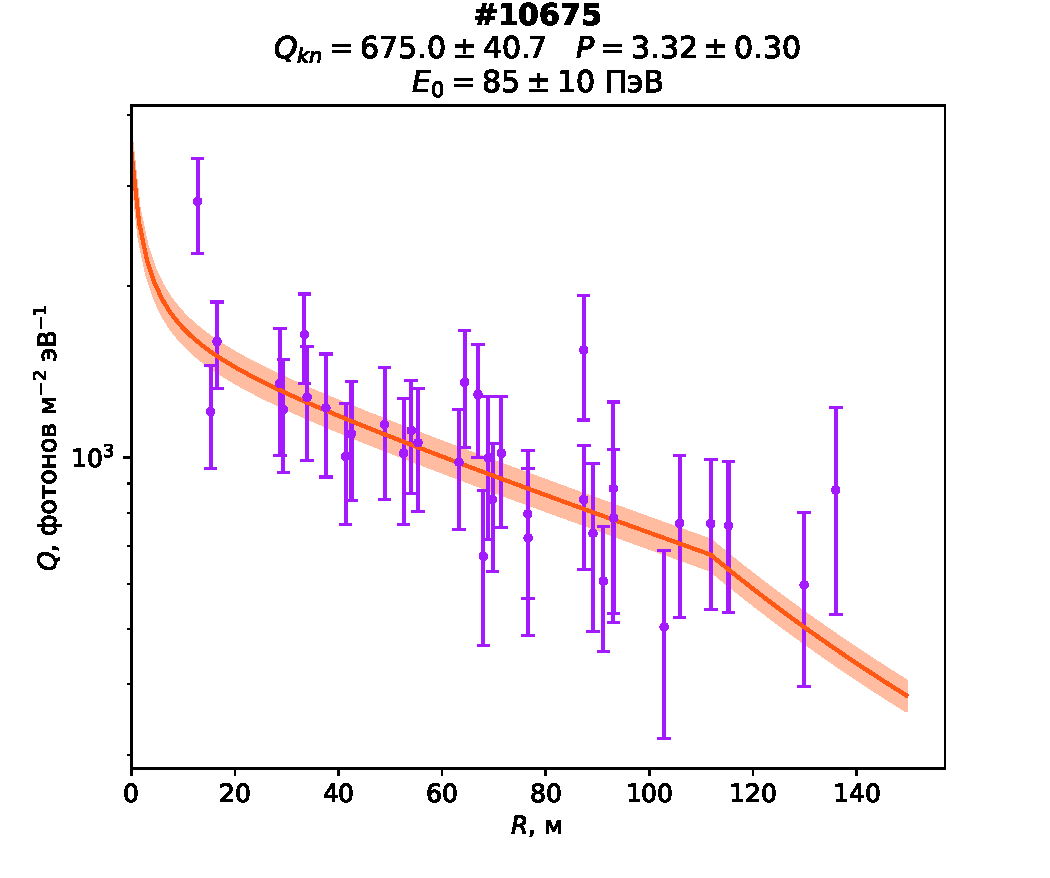
\includegraphics[width=0.9\columnwidth]{ldf-fit-10675}
	\caption{То же самое, что рис. \ref{pic:ldf-fit-example-1} для другого экспериментального события.}
	\label{pic:ldf-fit-example-2}
\end{figure}


\subsection{Определение параметров ливня}

Используя описанную процедуру фитирования для оценки оптимального значения и неопределённости каждого из параметров ФПР, можно, наконец, перейти к оценке параметров первичной частицы ливня. За рамками данной работы остаются вопросы связи энергии и массы первичной частицы, а также глубины максимума, с наблюдаемыми характеристиками ФПР. На этом этапе необходимо учитывать модельные неопределённости, то есть статистический зарактер зависимости параметров ФПР от исследуемых характеристик ливня.

В этом разделе ограничимся простым применением формулы для связи $E_0$ и $Q(R)$ \cite{Budnev2005}:

\begin{equation}
	\label{eq:E0-from-Q175}
	E \; [\text{ТэВ}] = 400 \cdot Q(175)^{0.95}
\end{equation}

Чтобы определить неопределённость $Q_{175}$, и как следствие $E$ с учётом оцененных неопределённостей параметров $Q_{kn}$ и $P$ сэмплируем каждый из них и вычислим среднее и стандартное отклонение по декартову произведению выборок (как видно из выражения (\ref{eq:tunka-25-ldf}), ФПР нетривиальным образом зависит от $P$).

Полученные энергии с соответствующими погрешностями приведены на рис. \ref{pic:ldf-fit-example-1} и \ref{pic:ldf-fit-example-2} вместе с параметрами ФПР. Погрешность определяется для каждого события отдельно, но в общем по двум примерам с различными энергиями и положениями оси относительно детектора её можно оценить в $5$ -- $10 \%$. Детальное исследование систематической инструментальной погрешности -- зависимость от энергии и положения ливня, высоты и ориентации установки -- будет предметом дальнейших изысканий.

Также следует качественно сравнить полученные величины с модельными погрешностями, которые могут быть найдены, например, в работе \cite[табл. 1]{Anokhina2007}. Для ливней с энергией $1$ -- $10$ ПэВ флуктуации $Q(150)$, например, оцениваются в $2$ -- $10 \%$, уменьшаясь с энергией и массой первичной частицы. Для событий с энергиями $\approx 80$ и $\approx 206$ ПэВ эти модельные неопределённости будут ещё меньше -- следовательно, особенно важным становится именно точное определение инструментальной погрешности.

